\ifprof
\else

\subsection{Introduction}
\subsubsection{Présentation}

\begin{figure}[!htb]
\begin{minipage}{0.5\textwidth}
Dans une problématique d'entretien du parc éolien, les techniciens sont appelés à monter et descendre plusieurs fois par jour des échelles pouvant mesurer jusqu'à 80 mètres. L'entreprise française Fixator, fabricant de treuils et de plateformes suspendues dans le domaine du bâtiment et des travaux publiques (BTP) depuis plus de 90 ans, a mis à profit son expérience pour concevoir un système autonome d'aide à la montée, Exolift. Ce système portatif sur batterie fonctionne indépendamment de l'éolienne (si le parc éolien est mis hors tension pour des raisons de sécurité, les techniciens de maintenance peuvent profiter pleinement de leur aide à la montée, contrairement aux systèmes installés à demeure sur l'échelle de l'éolienne). Exolift permet ainsi de réduire les temps d'arrêt des éoliennes. Exolift est également un équipement qui minimise l'investissement initial pour les exploitants des parcs éoliens car il s'utilise sur une simple sangle installée à demeure sur l'échelle, réduisant le temps d'installation et le coût matériel.
\end{minipage}
\begin{minipage}{0.5\textwidth}
\begin{center}
\includegraphics[width=0.8\textwidth]{images/2023_10_30_d11e80da56f59e3b3cdfg-02}
\caption{Exolift utilisé sur une échelle \label{fig1}}
\end{center}
\end{minipage}
\end{figure}


\subsubsection{Analyse structurelle}
D'une manière générale, l'Exolift utilise le phénomène d'adhérence entre la sangle et un galet motorisé. La sangle étant fixée à l'échelle, lorsque le galet va tourner, l'ensemble Exolift va alors se déplacer le long de la sangle et supporter une partie du poids de l'utilisateur à la montée, comme à la descente (figure \ref{fig1}).

Il est principalement constitué (figure \ref{fig2}) d'un cadre 1, d'un panneau de commande 2, d'une batterie 3 , d'un moteur électrique 4 , d'un réducteur avec renvoi d'angle 5 et d'un galet motorisé 6 . Le panneau de contrôle/commande permet à l'utilisateur d'obtenir des informations sur l'état du système (par le biais de 5 leds multicolores) et d'envoyer des ordres de commande (marche/arrêt via un interrupteur, monter/descendre via une manette de commande, arrêt d'urgence...). L'Exolift comporte également un axe dynamométrique 7, permettant de mesurer l'action mécanique de l'utilisateur sur l'Exolift, et un capteur à effet Hall au niveau de l'arbre du moteur permettant de mesurer la vitesse angulaire du moteur (uniquement pour des questions de sécurité). Un capteur de fin de course est positionné aux extrémités de l'échelle afin de stopper l'Exolift. Enfin, une option sur l'Exolift permet de le renvoyer à vide en haut ou en bas de l'échelle afin qu'une autre personne puisse l'utiliser. Toutes ces commandes et informations sont traitées par une carte électronique embarquée qui se charge de générer la commande du moteur tout en assurant la sécurité de l'utilisateur.

Le diagramme de définition des blocs (figure \ref{fig3}) présente les différents sous-systèmes et composants de l'Exolift. Le diagramme de blocs interne (figure 4) présente l'architecture de l'Exolift ainsi que les flux échangés entre les différents sous-systèmes. Un extrait du cahier des charges est présenté par le diagramme des exigences (voir figure \ref{DR6}).


\begin{figure}[!htb]
\begin{center}
\includegraphics[width=0.9\textwidth]{images/2023_10_30_d11e80da56f59e3b3cdfg-03}
\caption{À gauche, vue de l'Exolift suivant l'axe du galet (sans la batterie); à droite, vue de face avec la batterie \label{fig2}}
\end{center}
\end{figure}


\begin{figure}[!htb]
\begin{center}
\includegraphics[width=0.9\textwidth]{images/2023_10_30_d11e80da56f59e3b3cdfg-03(1)}
\caption{Diagramme de définition des blocs partiel de l'Exolift \label{fig3}}
\end{center}
\end{figure}



\begin{figure}[!htb]
\begin{center}
\includegraphics[width=0.9\textwidth]{images/2023_10_30_d11e80da56f59e3b3cdfg-04(1)}
\caption{Diagramme de blocs interne partiel de l'Exolift \label{fig4}}
\end{center}
\end{figure}


\fi

\question{Compléter la chaîne structurelle de l'Exolift du Document Réponse en précisant le nom des composants et la nature des flux échangés (I pour information, E pour énergie et $M$ pour matière).}



\ifprof
  \ifthenelse{\boolean{corrige}}{
  \begin{center}
  \includegraphics[width=1.0\textwidth]{images/CF_corrige}
  \end{center}  
  }
  {
  \begin{center}
  \includegraphics[width=1.0\textwidth]{images/2023_10_30_d11e80da56f59e3b3cdfg-17}
  \end{center}
  }

\else




\FloatBarrier
\subsection{ Étude du fonctionnement général du système}
\subsubsection{I.1 - Loi de commande}

\begin{objectif}
 analyser la génération de la consigne de vitesse (exigence 1.3.3.3).
\end{objectif}


\begin{figure}[!htb]
\begin{minipage}{0.6\textwidth}

Afin de garantir la sécurité de l'utilisateur et la bonne utilisation de son système, notamment en descente, les concepteurs ont mis en place une consigne de vitesse, de norme notée $v$, de l'Exolift qui dépend du poids $P_{u}$ (masse $m_{u}$ ) de l'utilisateur équipé. Cette loi de commande (figure \ref{fig5}), intégrée dans la carte de commande, prend en entrée la force de l'utilisateur sur l'Exolift, mesurée par l'axe dynamométrique, notée $F_{m}$.

Afin de prendre en compte les discontinuités de cette loi, l'utilisation d'une seule fonction conditionnelle est retenue : la fonction de Heaviside, notée $u$, définie telle que :

$$
\forall x<0, u(x)=0 \quad \text { et } \quad \forall x \geq 0, u(x)=1
$$
\end{minipage}
\begin{minipage}{0.4\textwidth}
\begin{center}
\includegraphics[width=0.9\textwidth]{images/2023_10_30_d11e80da56f59e3b3cdfg-04}
\caption{Consigne de vitesse de l'Exolift en fonction de la force $F_{m}$ \label{fig5}}
\end{center}
\end{minipage}
\end{figure}

\fi
\question{Quel est le comportement de l'Exolift en descente lorsque l'utilisateur se laisse pendre et ne touche pas l'échelle?}

\ifprof
\begin{texteCache}

Si l'utilisateur se laisse pendre et ne touche pas l'échelle, alors
  \(F_{m} = P_{u}\) et on lit alors \(v = 0\). L'Exolift est alors
  bloqué et l'utilisateur est à l'arrêt.

\end{texteCache}

\else
\fi
\question{Partant du point de vitesse de consigne B, en montée, quel sera le comportement de l'Exolift si l'utilisateur ralentit? Et s'il accélère?}

\ifprof
\begin{texteCache}

A partir du point B~:


\begin{itemize}
\item
  Si l'utilisateur ralentit alors l'Exolift va supporter un poids plus
  important, dépassant \(0,8\ P_{u}\) et alors se mettre à l'arrêt.
\item
  Si l'utilisateur accélère alors l'Exolift va supporter un poids moins
  important et sa vitesse va alors augmenter.
\end{itemize}

\end{texteCache}

\else


\fi
\question{Compléter l'expression de la loi de vitesse $v\left(F_{m}\right)$ :

$
v\left(F_{m}\right)=v_{\max } u\left(F_{m}-0,05 P_{u}\right) \pm \cdots
$

sous forme de combinaison linéaire de la fonction $u$ décalée (par exemple, $u\left(F_{m}-F_{1}\right)$ pour la fonction décalée de $F_{1}$ ) en fonction des vitesses $v_{\max }, v_{\min }$ et des différents taux du poids de l'utilisateur.}

\ifprof
\begin{texteCache}

\[\nu\left( F_{m} \right) = \nu_{\max}u\left( F_{m} - 0,05\ P_{u} \right) + \frac{\nu_{\min} - \nu_{\max}}{0,5\ P_{u}}F_{m}u\left( F_{m} - 0,3\ P_{u} \right) - \left( \frac{\nu_{\min} - \nu_{\max}}{0,5\ P_{u}}F_{m} + \nu_{\min} \right)u\left( F_{m} - 0,8\ P_{u} \right)\]

\end{texteCache}

\else



C'est cette loi $v\left(F_{m}\right)$ qui est implantée dans la carte de commande.

Dans la suite du sujet, seul le cas simple d'une consigne de vitesse constante sera étudié.
%
%\section{I.2 - Étude de l'opération de pesée}
%Objectif : analyser le déroulement de la pesée initiale (exigence 1.3.3.1).
%
%L'étude précédente a montré que la commande de l'Exolift dépend du poids de l'utilisateur $P_{u}$. C'est pourquoi avant toute utilisation de l'Exolift, une opération de pesée est effectuée. Pendant cette opération, l'utilisateur doit se suspendre pendant au moins 3 secondes afin que l'axe dynamométrique puisse mesurer $P_{u}$. Cette valeur sera ensuite comparée à des valeurs limites de réglage (valeurs minimale notée $F_{\min }$ et maximale notée $F_{\max }$ ) pour vérifier que la prise de mesure s'est exécutée correctement. Les diagrammes d'états suivants (figures 6 et 7 ) présentent la commande de l'Exolift permettant de réaliser la pesée, dont les évènements et actions sont précisés ci-dessous.
%
%\section{Évènements}
%ON : l'Exolift est alimenté
%
%OFF : l'Exolift est éteint
%
%Pmes $=0$ : la pesée n'est pas encore faite
%
%Pmes $=1:$ la pesée s'est bien déroulée
%
%défaut=1: la pesée ne s'est pas bien effectuée $r=1$ : une demande de renvoi de l'Exolift a été effectuée
%
%$\mathrm{m}=0$ : la manette est relâchée (figure 2)
%
%$\mathrm{m}=1$ : la manette est enfoncée
%
%$\mathrm{m}=$ haut : la manette est levée
%
%$\mathrm{m}=$ bas : la manette est baissée
%
%\section{Actions}
%allumer une led: cette action est monostable, c'est-à-dire que lorsqu'elle n'apparaît pas dans un état, la led est éteinte. Les leds peuvent s'allumer en vert ou en rouge.
%
%BIP : un BIP sonore est émis.
%
%La durée des transitions est négligée et lorsque l'utilisateur se suspend sans toucher l'échelle, le poids mesuré $P_{u}$ sera considéré comme compris entre $F_{\min }$ et $F_{\max }$.
%
%Le scénario étudié est le suivant :
%
%\begin{itemize}
%  \item à $t=0 \mathrm{~s}$, l'utilisateur appuie sur ON et se suspend;
%
%  \item à $t=1 \mathrm{~s}$, il enfonce la manette;
%
%  \item à $t=2 \mathrm{~s}$, il remonte sur l'échelle pour vérifier son matériel, la valeur moyenne mesurée de $P_{u}$ sera donc inférieure à $F_{\text {min }}$;
%
%  \item à $t=5 \mathrm{~s}$, il se suspend;
%
%  \item à $t=8 \mathrm{~s}$, il enfonce la manette;
%
%  \item à $t=12 \mathrm{~s}$, il remonte sur l'échelle.
%
%\end{itemize}
%
%Q5. Compléter le DR2 en indiquant, pour chaque instant, les leds allumées ainsi que les valeurs de Pmes et défaut.
%
%\begin{center}
%\includegraphics[width=0.9\textwidth]{images/2023_10_30_d11e80da56f59e3b3cdfg-06}
%\end{center}
%
%Figure 6 - Diagramme d'états de la commande de l'Exolift
%
%\begin{center}
%\includegraphics[width=0.9\textwidth]{images/2023_10_30_d11e80da56f59e3b3cdfg-06(1)}
%\end{center}
%
%Figure 7 - Diagramme d'états de l'état composite pesée
%
\subsection{Étude de la chaîne d'information}\label{II}


\begin{objectif}
Mettre en place le traitement des informations reçues de l'axe dynamométrique afin de les rendre utilisables par la carte de commande.
\end{objectif}

L'effort de l'utilisateur sur l'Exolift $F_{m}$, permettant d'imposer la commande de vitesse de l'Exolift, est mesuré à l'aide d'un axe dynamométrique. Cette action mécanique déforme l'axe dynanométrique. Cette déformation est mesurée à l'aide de deux jauges d'extensiométrie (jauges de déformation) collées sur un arbre. Le signal délivré par l'axe dynanométrique est une tension liée à l'effort recherché.

Dans cette partie, l'étalonnage du capteur, puis le filtrage de sa sortie seront analysés et, ensuite, les différentes données enregistrées lors d'un étalonnage seront exploitées.
%
\subsubsection{Étalonnage de l'axe dynanométrique}\label{II.1}

\begin{objectif}
Déterminer le modèle de comportement du capteur afin de déterminer la relation entre la tension sortie du capteur et l'effort $F_{m}$ recherché (exigence 1.3.3.1.1).
\end{objectif}


Un étalonnage, réalisé sur le site de production, permet d'obtenir la relation entre l'effort $F_{m}$ et le signal de sortie du capteur. La figure \ref{fig8} présente les résultats d'un étalonnage réalisé sur l'axe dynanométrique de l'Exolift. Ce graphique montre que la relation entre la tension de sortie du capteur et l'effort mesuré peut être approximée par une loi affine, qui sera considérée valide sur toute la plage d'utilisation de l'axe dynamométrique. Il est donc proposé ici de programmer une régression linéaire.

Pour réaliser la régression linéaire, la méthode des moindres carrés sera utilisée. Elle consiste à modéliser au mieux les points expérimentaux par une droite (figure \ref{fig9}).

\begin{figure}[!htb]
\begin{minipage}{0.5\textwidth}
\begin{center}
\includegraphics[width=0.9\textwidth]{images/2023_10_30_d11e80da56f59e3b3cdfg-07(1)}
\caption{Résultat d'un étalonnage \label{fig8}}
\end{center}
\end{minipage}
\begin{minipage}{0.5\textwidth}
\begin{center}
\includegraphics[width=0.9\textwidth]{images/2023_10_30_d11e80da56f59e3b3cdfg-07}
\caption{Droite obtenue par la méthode des moindres carrés \label{fig9}}
\end{center}
\end{minipage}
\end{figure}



L'équation de la droite sera notée $u=a P+b$. Pour chaque mesure, le poids pendu sera noté $P_{i}$, la tension mesurée $u_{i}$ et l'écart entre la tension mesurée et la tension modélisée sera noté $\varepsilon_{i}$ (figure 9).

Soit $N$ le nombre de mesures réalisées pendant l'étalonnage $(N=5$ sur la figure 9 ), la méthode des moindres carrés consiste à trouver les valeurs de $a$ et $b$ qui minimisent le réel :

$$
S=\sum_{i=0}^{i=N-1} \varepsilon_{i}^{2}
$$

\fi
\question{Donner l'expression de $\varepsilon_{i}$ en fonction de $a, b, P_{i}$ et de $u_{i}$.}
\ifprof
\begin{texteCache}

\[\varepsilon_{i} = u_{i} - u\left( P_{i} \right) = u_{i} - a*P_{i} - b\]

Remarque~: \(\varepsilon_{i}\) étant sommé au carré dans \(S\), on
pouvait aussi définir
\(\varepsilon_{i} = u\left( P_{i} \right) - u_{i}\)

\end{texteCache}
\else


La résolution de cette minimisation permet de trouver les expressions de $a$ et $b$ :

$$
a=\frac{N S_{P u}-S_{P} S_{u}}{N S_{P P}-S_{P}^{2}} \quad b=\frac{S_{P} S_{P u}-S_{u} S_{P P}}{S_{P}^{2}-N S_{P P}}
$$

avec :

$$
S_{P}=\sum_{i=0}^{i=N-1} P_{i} \quad S_{u}=\sum_{i=0}^{i=N-1} u_{i} \quad S_{P P}=\sum_{i=0}^{i=N-1} P_{i}^{2} \quad S_{P u}=\sum_{i=0}^{i=N-1} P_{i} u_{i}
$$

\paragraph{Notations et hypothèses}
\begin{itemize}
  \item Les bibliothèques numpy et matplotlib.pyplot ont été importées : import numpy as np et import matplotlib.pyplot as plt.

  \item Les poids $P_{i}$ sont stockés dans un tableau numpy de longueur $N$, noté $\mathrm{P}$ : $\mathrm{P}=\mathrm{np}$. array $([\mathrm{PO}, \mathrm{P} 1, \ldots])$.

  \item Les tensions $u_{i}$ sont stockées dans un tableau numpy de longueur $N$, noté u : $\mathrm{u}=\mathrm{np}$. array $([\mathrm{u} 0, \mathrm{u} 1, \ldots])$.

  \item La longueur $N$ n'est pas affectée.

\end{itemize}

\paragraph{Fonctions de la bibliothèque numpy}
\begin{itemize}
  \item La fonction $n p \cdot \operatorname{dot}(X, Y)$ donne le produit matriciel; lorsque $X$ et $Y$ sont deux tableaux de longueur $N, \mathrm{np} \cdot \operatorname{dot}(\mathrm{X}, \mathrm{Y})$ a la même valeur que le produit scalaire entre $\mathrm{X}$ et $\mathrm{Y}$.

  \item La fonction $n p . \operatorname{sum}(X)$ donne la somme des éléments du tableau $X$.

  \item La fonction np.ones $(\mathrm{N})$ donne un tableau numpy de longueur $N$ où tous les éléments ont pour valeur 1.

\end{itemize}


\fi

\question{Proposer deux instructions permettant d'affecter les variables SPP puis SPu représentant $S_{P P}$ et $S_{P u}$ en utilisant les tableaux $\mathrm{P}$ et $\mathrm{u}$, les fonctions de numpy et sans faire de boucle.}

\ifprof
\begin{texteCache}

\begin{lstlisting}

SPP=np.dot(P,P)
SPu=np.dot(P,u)

\end{lstlisting}

\end{texteCache}
\else

\fi

\question{Proposer deux instructions permettant d'affecter les variables SP puis Su représentant $S_{P}$ et $S_{u}$ en utilisant les tableaux $P$ et $u$, les fonctions de numpy et sans faire de boucle.}

\ifprof
\begin{texteCache}

\begin{lstlisting}
SP=np.sum(P)
Su=np.sum(u)
\end{lstlisting}


\end{texteCache}
\else

\fi

\question{Proposer des instructions permettant d'affecter les variables a puis b représentant $a$ et $b$ en utilisant les tableaux $\mathrm{P}$ et $\mathrm{u}$ et les variables précédemment définies.}

\ifprof
\begin{texteCache}

\begin{lstlisting}
N=len(P)
a=(N*SPu-SP*Su)/(N*SPP-SP**2)
b=(SP*SPu-SPP*Su)/( SP**2-N*SPP)
\end{lstlisting}

\end{texteCache}
\else

\fi

\question{En considérant les variables a et b affectées, proposer des instructions permettant de tracer uniquement les points et la droite de la figure \ref{fig9}. Dans la fonction plot, l'argument supplémentaire ' $O$ ' permet de ne pas relier les points par une droite.}


\ifprof
\begin{texteCache}
\begin{lstlisting}
  plt.new()

  plt.plot(P,u,'o')

  plt.plot(P,a*P+b)

  plt.show()
\end{lstlisting}



\end{texteCache}
\else



\subsubsection{Filtrage de la tension de sortie du capteur}


\begin{objectif}:
Analyser deux types de filtre (exigence 1.3.3.1.2).
\end{objectif}

Comme le montre la figure \ref{fig10}, la tension de sortie du capteur est bruitée. Afin d'améliorer le comportement de l'Exolift, un filtrage de la sortie du capteur est nécessaire. Deux méthodes de filtrage vont être programmées : la moyenne glissante et le filtre passe-bas.

\begin{figure}[!htb]
\begin{center}
\includegraphics[width=0.9\textwidth]{images/2023_10_30_d11e80da56f59e3b3cdfg-09(1)}
\caption{Signal brut du capteur \label{fig10}}
\end{center}
\end{figure}


\paragraph{Notations et hypothèses}

Les notations et hypothèses de la partie \ref{II}-\ref{II.1} sont complétées par :

\begin{itemize}
  \item les tensions filtrées $u_{i}^{f}$ sont stockées dans un tableau numpy de longueur $N$, noté uf : uf=np. array ( [uf 0, uf $1, \ldots])$;

  \item les instants $t_{i}$ sont stockés dans un tableau numpy de longueur $N$, noté temps : temps $=n p$. array $([t 0, t 1, \ldots])$.

\end{itemize}

\paragraph{Filtrage par moyenne glissante}

Cette méthode consiste à prendre la moyenne des mesures précédentes. $n$ est le nombre de mesures utilisées pour calculer la moyenne. Il est appelé ordre de la moyenne glissante. La moyenne glissante s'obtient alors par :

$$
\text { si } i<n-1, u_{i}^{f}=\sum_{k=0}^{k=i} \frac{u_{k}}{i+1} \quad \text { ou } \quad \text { si } i \geq n-1, u_{i}^{f}=\sum_{k=i-n+1}^{k=i} \frac{u_{k}}{n}
$$


\fi

\question{Compléter le tableau du document réponse en utilisant la méthode de la moyenne glissante pour $n=3$ avec le tableau u donné contenant 5 éléments.}
\ifprof
  \ifthenelse{\boolean{corrige}}{
  \renewcommand{\arraystretch}{3}
  \begin{center}
\begin{tabular}{p{0.1\textwidth}p{0.1\textwidth}p{0.1\textwidth}p{0.1\textwidth}p{0.1\textwidth}p{0.1\textwidth}}
\hline
\(\mathbf{i}\) & 0 & 1 & 2 & 3 & 4\\
\hline
\(\mathbf{u}_{\mathbf{i}}\) & -2 & 0 & -1 & 2,5 & 3\\
\hline
\(\mathbf{u}_{\mathbf{i}}^{\mathbf{f}}\) & -2 & -1 & -1 & 0,5 &
1,5\\
\hline
\end{tabular}
 \end{center}
}
{
\renewcommand{\arraystretch}{3}
 \begin{center}
\begin{tabular}{p{0.1\textwidth}p{0.1\textwidth}p{0.1\textwidth}p{0.1\textwidth}p{0.1\textwidth}p{0.1\textwidth}}
\hline
\(\mathbf{i}\) & 0 & 1 & 2 & 3 & 4\\
\hline
\(\mathbf{u}_{\mathbf{i}}\) & -2 & 0 & -1 & 2,5 & 3\\
\hline
\(\mathbf{u}^f_{\mathbf{i}}\)&  &  &  &  &\\
\hline
\end{tabular}
 \end{center}

}

\else

\fi

\question{Créer la fonction filtre\_mg $(u, n)$ qui prend pour argument $u$, un tableau de mesures à filtrer et n l'ordre de la moyenne glissante et renvoie un tableau de mesures filtrées par cette méthode.}

\ifprof
\begin{texteCache}
\begin{lstlisting}
def filtre_mg(u,n):
	uf=np.ones(len(u))
	for i in range(len(u)):
		s=0
		if i< n-1:
			for j in range(i+1):
				s+=u[j]
			uf[i]=(s/(i+1))
		else:
			for j in range(i-n+1,i+1):
				s+=u[j]
			uf[i]=(s/n)
	return uf
	
	
def filtre_mg(u,n):
	uf=np.ones(len(u))
	for i in range(len(u)):
		if i< n-1:
			uf[i]=(np.sum(u[:i+1])/(i+1))
		else:
			uf[i]=(np.sum(u[i-n+1:i+1])/n)
	return uf
\end{lstlisting}



\end{texteCache}
\else



%
La figure \ref{fig11} présente le résultat du filtrage par la moyenne glissante pour différentes valeurs de $n$.

%
\begin{figure}[!htb]
\begin{center}
\includegraphics[width=0.9\textwidth]{images/2023_10_30_d11e80da56f59e3b3cdfg-09}
\caption{Signal filtré par la méthode de la moyenne glissante pour différents ordres \label{fig11}}
\end{center}
\end{figure}

%Figure 11 - Signal filtré par la méthode de la moyenne glissante pour différents ordres
\fi
\question{Quelle est l'influence de l'ordre $n$ sur la qualité du filtrage ?}
\ifprof
\begin{texteCache}

Si \(n\) est trop faible, alors le bruit de mesure est atténué mais
  non supprimé (cas où \(n = 20\)). Par contre si \(n\) est trop grand,
  alors c'est toute la courbe qui est lissée, faisant disparaitre
  également les oscillations propres du signal.
  
  
    \vspace{2cm}
  \end{texteCache}
\else

\paragraph{Filtrage par filtre passe-bas}

Dans le cas d'un filtre passe-bas d'ordre 1 , cette méthode revient à résoudre l'équation différentielle suivante :

$$
\tau \frac{d u_{f}(t)}{d t}+u_{f}(t)=u(t)
$$

où $f=\frac{1}{2 \pi \tau}$ est la fréquence de coupure, $u(t)$ est le signal à filtrer, $u_{f}(t)$ le signal filtré et $t$ le temps.

\fi


\question{Donner l'expression de $u_{i+1}^{f}$ en fonction de $u_{i}^{f}, u_{i}, t_{i+1}, t_{i}$ et de $\tau$ en utilisant la méthode d'Euler explicite. Proposer une valeur pour $u_{0}^{f}$.}

\ifprof
\begin{texteCache}
La méthode d'Euler explicite revient à approximer la dérivé
  \(\frac{du_{f}(t)}{\text{dt}}\) par
  \(\frac{u_{i + 1}^{f} - u_{i}^{f}}{t_{i + 1} - t_{i}}\). L'équation
  différentielle devient donc~:

\[\tau*\frac{u_{i + 1}^{f} - u_{i}^{f}}{t_{i + 1} - t_{i}} + u_{i}^{f} = u_{i}\]

soit

\[u_{i + 1}^{f} = u_{i}^{f} + \frac{\left( t_{i + 1} - t_{i} \right)\left( u_{i} - u_{i}^{f} \right)}{\tau}\]

Initialement on prendre \(u_{0}^{f} = u_{0}\)

  \vspace{2cm}
\end{texteCache}
\else

\fi

\question{Créer la fonction filtre\_pb (u,temps,f) qui prend pour argument un tableau u des mesures à filtrer, un tableau temps, de même dimension, représentant le temps et $f$ la fréquence de coupure du filtre passe-bas et qui renvoie un tableau des mesures filtrées par cette méthode.}


\ifprof
\begin{texteCache}

\begin{lstlisting}
def filtre_pb(u,temps,f):
	uf=np.ones(len(u))
	uf{[0]=u[0]
 	for i in range(len(u)-1):
		uf[i+1]=uf[i]+f*2*np.pi()*(temps[i+1]-temps[i])*(u[i]-uf[i])
	return uf
\end{lstlisting}

  \vspace{2cm}

\end{texteCache}
\else



%
La figure \ref{fig12} présente le résultat du filtrage passe-bas pour différentes valeurs de $f$.

\begin{figure}[!htb]
\begin{center}
\includegraphics[width=0.9\textwidth]{images/2023_10_30_d11e80da56f59e3b3cdfg-10(1)}
\caption{Signal filtré par un filtre passe-bas pour différentes fréquences de coupure \label{fig12}}
\end{center}
\end{figure}



\fi

\question{Quelle est l'influence de la fréquence de coupure $f$ sur la qualité du filtrage ?}

\ifprof
\begin{texteCache}

 Plus la fréquence de coupure est faible, plus les hautes fréquences
  sont atténuées. Il faut donc la choisir judicieusement pour réduite
  les oscillations indésirables (qui ont une fréquence élevée) et
  conserver la fréquence propre.
  \vspace{2cm}
\end{texteCache}
\else


\paragraph{Comparaison des méthodes}

La figure \ref{fig13} montre le résultat du filtrage par les deux méthodes vues précédemment.

\begin{figure}[!htb]
\begin{center}
\includegraphics[width=0.9\textwidth]{images/2023_10_30_d11e80da56f59e3b3cdfg-10}
\caption{Signal filtré par les deux méthodes \label{fig13}}
\end{center}
\end{figure}

\fi

\question{Comparer la complexité temporelle asymptotique des deux méthodes.}

\ifprof
\begin{texteCache}

 La méthode du filtrage par moyennes glissante est de complexité
  \(o(n*N)\) alors que la méthode de filtrage par filtre passe bas est
  de complexité \(o(N)\).

\end{texteCache}
\else





\subsection{Étude de la chaîne d'énergie}

\begin{objectif}
Modéliser le comportement dynamique du système afin d'analyser son comportement face à une perturbation (exigence 1.3.2).
\end{objectif}

Le schéma-blocs fonctionnel de la figure 14 présente la modélisation du comportement de l'Exolift.

\begin{figure}[!htb]
\begin{center}
\includegraphics[width=0.9\textwidth]{images/2023_10_30_d11e80da56f59e3b3cdfg-12(1)}
\caption{Schéma-blocs fonctionnel de l'Exolift \label{fig14}}
\end{center}
\end{figure}


\subsubsection{Dynamique du système}

\begin{objectif}
Déterminer la fonction de transfert associée au comportement dynamique du système.
\end{objectif}


\paragraph{Paramétrage et modélisation}


\begin{figure}[!htb]
\begin{center}
\includegraphics[width=0.9\textwidth]{images/2023_10_30_d11e80da56f59e3b3cdfg-12}
\caption{Représentation des efforts lors d'une montée d'échelle et graphe de structure associé (les liaisons en pointillés correspondent aux hypothèses de modélisation retenues, les noeuds en gris sont des sous-systèmes de l'Exolift) \label{fig15}}
\end{center}
\end{figure}

La figure \ref{fig15} présente les seuls efforts pris en compte dans la modélisation. On considère que :

\begin{itemize}
  \item le référentiel, de base $(\vec{x}, \vec{y}, \vec{z})$, lié à l'échelle est considéré comme fixe et galiléen;

  \item la verticale ascendante est modélisée par le vecteur $\vec{z}$;

  \item l'accélération de la pesanteur est notée $\vec{g}=-g \vec{z}$ avec $g=9,81 \mathrm{~m} \cdot \mathrm{s}^{-2}$;

  \item l'utilisateur équipé, de masse $m_{u}$, exerce un effort $\overrightarrow{F_{u \rightarrow e c}}=-F_{u \rightarrow e c} \vec{z}$ sur l'échelle;

  \item I'Exolift, de masse $m_{e}$, est soumis à l'effort de la sangle noté $\overrightarrow{F_{s \rightarrow e x}}=F_{s \rightarrow e x} \vec{z}$. II a un mouvement de translation rectiligne le long de l'échelle (suivant la direction $\vec{z}$ );
  
  \item les autres masses sont négligées ;

  \item l'utilisateur étant relié à l'Exolift par un mousqueton, directement lié à l'axe dynamométrique, l'utilisateur et l'Exolift se déplacent à la même vitesse par rapport à l'échelle, notée $\overrightarrow{V(t)}=v(t) \vec{z}$. L'effort mesuré par l'axe dynamométrique, à savoir l'effort de l'utilisateur sur l'Exolift, est noté $\overrightarrow{F_{u \rightarrow e x}}=-F_{u \rightarrow e x} \vec{z}$.

\end{itemize}



\fi
%Q21. En isolant l'Exolift et l'utilisateur et en précisant le théorème utilisé, déterminer la relation entre les efforts $F_{s \rightarrow e x}, F_{u \rightarrow e c}$, la vitesse $v(t)$ et les données.

\question{Isoler l'Exolift et l'utilisateur (donc tout sauf l'échelle) et faire un bilan d'action mécanique extérieur en résultante en projection sur $\overrightarrow{z}$.}

\ifprof
\begin{texteCache}

 On isole l'ensemble \{Exolift + Utilisateur\} et on effectue un bilan des forces selon $\overrightarrow{z}$ :


\begin{itemize}
\item
  \(\overrightarrow{F_{s \rightarrow ex}}.\overrightarrow{z} = F_{s \rightarrow ex}\)
\item
  \(\overrightarrow{F_{ec \rightarrow u}}.\overrightarrow{z} = - \overrightarrow{F_{u \rightarrow ec}}.\overrightarrow{z} = F_{u \rightarrow ec}\)
\item
  \(\overrightarrow{P_{g \rightarrow chassis}}.\overrightarrow{z} = - m_{e}g\)
\item
  \(\overrightarrow{P_{g \rightarrow utilisateur}}.\overrightarrow{z} = - m_{u}g\)
\item
  La glissière entre le châssis et la sangle ne transmet pas d'effort
  suivant \(\overrightarrow{z}\)

\end{itemize}

\end{texteCache}
\else



Le théorème de la résultante dynamique appliqué à un ensemble $E$ de masse $m$ et de centre d'inertie $G$ en mouvement dans un référentiel galiléen $R$ est donné par : 

\begin{align}\label{PFD}
 \overrightarrow{F}_{ext\to E}=m\cdot \overrightarrow{a}(G\in E/R)
\end{align}


\fi
\question{En projetant l'équation \ref{PFD} sur $\overrightarrow{z}$ appliqué à E= \{Exolift + Utilisateur\} déterminer la relation entre les efforts $F_{s \rightarrow e x}, F_{u \rightarrow e c}$, la vitesse $v(t)$ et les données.}


\ifprof
\begin{texteCache}

 \[F_{s \rightarrow ex} + F_{u \rightarrow ec\ } - \left( m_{u} + m_{e} \right)g = \left( m_{u} + m_{e} \right)\dot{v}(t)\]
 
 \vspace{3cm}

\end{texteCache}
\else




\subsubsection{Modélisation de la motorisation}
Le moteur électrique présent dans l'Exolift peut-être modélisé par les équations suivantes :

$$
u_{m}(t)=R_{m} i_{m}(t)+L_{m} \frac{\mathrm{d} i_{m}(t)}{\mathrm{d} t}+e(t) ; \quad J_{e} \frac{\mathrm{d} \omega_{m}(t)}{\mathrm{d} t}=c_{m}(t)+c_{r}(t) ; \quad e(t)=K_{e} \omega_{m}(t) ; \quad c_{m}(t)=K_{c} i_{m}(t) .
$$

\begin{center}
\begin{tabular}{|ll|}
\hline
Notations du moteur &  \\
\hline
$u_{m}:$ tension d'alimentation du moteur & $R_{m}=0,086 \Omega:$ résistance aux bornes du moteur \\
$i_{m}:$ courant circulant dans le moteur & $L_{m}=0,305 \mathrm{mH}:$ inductance des bobines du moteur \\
$e:$ force contre-électromotrice du moteur & $J_{e}:$ inertie équivalente de l'ensemble \{arbre moteur, \\
$\omega_{m}:$ vitesse de rotation de l'arbre moteur & réducteur, galet\} ramenée sur l'arbre moteur \\
$c_{m}:$ couple disponible sur l'arbre moteur & $K_{e}=0,071 \mathrm{~V} \cdot \mathrm{s} \cdot \mathrm{rad}^{-1}:$ constante électrique \\
$c_{r}:$ couple résistant & $K_{c}=0,071 \mathrm{~N} \cdot \mathrm{m} \cdot \mathrm{A}^{-1}:$ constante de couple \\
\hline
\end{tabular}
\end{center}

L'arbre du moteur a un moment d'inertie suivant son axe de rotation $J_{m}=1,9 \cdot 10^{-4} \mathrm{~kg} \cdot \mathrm{m}^{2}$. II est relié à un réducteur avec renvoi d'angle de moment d'inertie $J_{r}$, ramené à son arbre de sortie, tel que $J_{r}=1,9 \cdot 10^{-2} \mathrm{~kg} \cdot \mathrm{m}^{2}$ et de rapport de réduction $\lambda=\frac{\omega_{r}}{\omega_{m}}=\frac{1}{30}$ avec $\omega_{r}$ la vitesse de rotation en sortie du réducteur. La sortie du réducteur est directement reliée au galet d'entraînement de la sangle, de rayon $R_{g}=0,03 \mathrm{~m}$, de masse $m_{g}=0,093 \mathrm{~kg}$ et d'inertie $J_{g}=62,628 \mathrm{~kg} \cdot \mathrm{mm}^{2}$. On précise que l'Exolift a une masse $m_{e}=11,5 \mathrm{~kg}$ et que l'utilisateur équipé ne peut pas avoir une masse supérieure à $130 \mathrm{~kg}$.

\paragraph{Hypothèses et notations}


\begin{itemize}
  \item Les masses de l'ensemble \{arbre moteur, réducteur, galet\} sont négligeables, seules leurs inerties seront prises en compte pour le calcul de l'énergie cinétique de cet ensemble.

  \item Les liaisons sont parfaites.

  \item Le rendement du réducteur est unitaire.

  \item Le contact entre le galet et la sangle se fait sans glissement.

  \item La transformée de Laplace d'une fonction temporelle $f(t)$ sera notée $F(p)=\mathcal{L}[f(t)]$.

\end{itemize}


\fi

\question{Dans les conditions de Heaviside, compléter les blocs grisés du schéma-blocs du DR4 modélisant le comportement du moteur électrique.}

\ifprof


  \ifthenelse{\boolean{corrige}}{
  \begin{center}
  \includegraphics[width=1.0\textwidth]{media/image3.png}
  \end{center}  
  }
  {
  \begin{center}
  \includegraphics[width=1.0\textwidth]{images/DR5_schema_bloc0}
  \end{center}
  }


\begin{texteCache}
 
 \vspace{3.5cm}

\end{texteCache}
\else

Une approche énergétique permet de déterminer l'inertie  équivalente \(J_{e}\) de l'ensemble \{arbre moteur, réducteur, galet\} ramenée sur l'arbre moteur.

\[J_{e} = J_{m} + \left( J_{g} + J_{r} \right)\lambda^{2}\]



\fi

\question{Déterminer l'expression numérique de l'inertie équivalente $J_{e}$ de l'ensemble \{arbre moteur, réducteur, galet\} ramenée sur l'arbre moteur.}

\ifprof
\begin{texteCache}

AN~:
\(J_{e} = 1,9 \times 10^{- 4} + \frac{\left( 62,6 \times 10^{- 6} + 1,9 \times 10^{- 2} \right)}{30^{2}} = 2,1 \times 10^{- 4}\text{kg.}m^{2}\)
 
 \vspace{1.5cm}

\end{texteCache}
\else


 En appliquant le théorème énergie-puissance à l'ensemble \{arbre moteur, réducteur, galet\}, on obtient la relation entre \(c_{m}\),
  \(F_{s \rightarrow ex}\), la vitesse \(v(t)\) et les données, on obtient,


$$J_{e}{\dot{\omega}}_{m} =C_{m} + R_{g}\lambda F_{s \rightarrow ex}$$

\fi

\question{En utilisant les résultats des questions précédentes et le schéma-blocs complété précédemment, déterminer l'expression de $J_{eq}$ en fonction de $J_{e}, m_{e}, m_{u}, \lambda$ et de $R_{g}$.}

\ifprof
\begin{texteCache}

 D'après le schéma bloc,
  \(\Omega_{m}\left( p \right) = \frac{1}{J_{\text{eq}}p}\left( C_{m} - R_{g}\lambda\left( F_{u \rightarrow \text{ex}} - P_{\text{ex}} - P_{u} \right) \right) \Rightarrow J_{\text{eq}}{\dot{\omega}}_{m}\left( t \right) = C_{m} - R_{g}\lambda\left( F_{u \rightarrow \text{ex}} - P_{\text{ex}} - P_{u} \right)\)

  Or d'après l'équation précdente


\[J_{e}{\dot{\omega}}_{m} = C_{m} + R_{g}\lambda F_{s \rightarrow \text{ex}}\]

Et en remplacent \(F_{s \rightarrow ex}\) à partir de la relation déterminée précédemment

\[J_{e}{\dot{\omega}}_{m} = C_{m} + R_{g}\lambda\left( \left( m_{u} + m_{e} \right)\dot{v} + \left( m_{u} + m_{e} \right)g - F_{u \rightarrow \text{ec}\ } \right)\]

\[\Rightarrow J_{e}{\dot{\omega}}_{m} - R_{g}\lambda\left( m_{u} + m_{e} \right)\dot{v} = C_{m} - R_{g}\lambda\left( F_{u \rightarrow \text{ec}\ } - P_{\text{ex}} - P_{u} \right)\]

\[\Rightarrow \left( J_{e} - R_{g}^{2}\lambda ²\left( m_{u} + m_{e} \right) \right){\dot{\omega}}_{m} = C_{m} - R_{g}\lambda\left( F_{u \rightarrow \text{ec}\ } - P_{\text{ex}} - P_{u} \right)\]

Donc par identification~:

\[J_{\text{eq}} = J_{e} - R_{g}^{2}\lambda ^2\left( m_{u} + m_{e} \right)\]
 
 \vspace{1.5cm}

\end{texteCache}
\else


\fi

\question{Déterminer l'expression littérale de la fonction de transfert $H_{pert}(p)=\frac{-V(p)}{F_{u \rightarrow e c}(p)}$ sous forme canonique en considérant les autres entrées nulles.}

\ifprof
\begin{texteCache}

\[H_{\text{pert}}\left( p \right) = R_{g}^{2}\lambda^{2}\frac{\frac{1}{J_{\text{eq}}p}}{1 + \frac{K_{c}K_{e}}{\left( R_{m} + L_{m}p \right)J_{\text{eq}}p}} = R_{g}^{2}\lambda^{2}\frac{R_{m} + L_{m}p}{\left( R_{m} + L_{m}p \right)J_{\text{eq}}p + K_{c}K_{e}}\]

\[H_{\text{pert}}\left( p \right) = \frac{R_{g}^{2}\lambda^{2}R_{m}}{K_{c}K_{e}}\ \frac{1 + \frac{L_{m}}{R_{m}}p}{1 + \frac{R_{m}J_{\text{eq}}}{K_{c}K_{e}}p + \frac{L_{m}J_{\text{eq}}}{K_{c}K_{e}}p^{2}}\]


 
 \vspace{1.5cm}

\end{texteCache}
\else




\subsubsection{Analyse de la stabilité}


On donne l'expression numérique de $H_{p e r t}(p)$ :

$$
H_{\text {pert }}(p)=1,7 \times 10^{-5} \times \frac{1+3,5 \times 10^{-3} p}{1+\frac{2 \times 0,65}{218} p+\frac{p^{2}}{218^{2}}}
$$


\fi

\question{Sur le document réponse, réaliser les tracés des diagrammes de Bode asymptotiques et réels de $H_{pert}(j \omega)$.}


\ifprof
\begin{texteCache}

%

Cette fonction  de transfert se décompose en $H_{pert}=H_1(p)\times H_2(p)$

\begin{itemize}
\item $H_1(p)=\dfrac{1,7 \times 10^{-5}}{1+\frac{2 \times 0,65}{218} p+\frac{p^{2}}{218^{2}}}$ : on choisit $\omega_1=218 rad/s$ la pulsation propre du second ordre avec $G_{db}(\omega \to 0)=20log(1,7 \times 10^{-5})\approx -95,4dB$
\item $H_2(p)=1+3,5 \times 10^{-3} p$ : on choisit $\omega_2=\dfrac{1}{\tau_2}=\dfrac{1}{3,5 \times 10^{-3}}\approx 285,7 rad/s$.
\end{itemize}

\renewcommand{\arraystretch}{3}

\begin{center}
\begin{tabular}{|p{2.cm}|p{1.5cm}|p{1.cm}|c|p{1.5cm}|p{1.cm}|c|p{1.5cm}|p{1.cm}|}
\hline 
$\omega$& \multicolumn{2}{c|}{$0\to \omega_1$}   & $\omega_1$ &  \multicolumn{2}{c|}{$\omega_1\to \omega_2$}  & $\omega_2$ &   \multicolumn{2}{c|}{$\omega_2 \to \infty$}\\ 
\hline 
Tracé asymptotique &Gain ($dB/dec$) & $\varphi (^\circ)$ & Gain ($dB$) & Gain ($dB/dec$) & $\varphi (^\circ)$ & Gain ($dB$) & Gain ($dB/dec$) & $\varphi (^\circ)$  \\ 
\hline 
$H_1(p)$ & $0$&$0$&$-95,4$&$-40$ & $-180$ & $-$ & $-40$ & $-180$  \\ 
\hline 
$H_2(p)$ & $0$& $0$& $0$ & $0$ & $00$ & $0$ & $+20$ & $+90$  \\ 
\hline 
\hline
$H_{pert}(p)$ &$0$& $0$ &$-95,4$ & $-40$ & $-180$ & $-$ & $-20$ & $-90$  \\ 
\hline 
\end{tabular} 
\end{center}


\end{texteCache}



 \ifthenelse{\boolean{corrige}}{
 \begin{center}
 \includegraphics[width=1.0\textwidth]{images/bode_total2}
 \end{center}
 }
 {
  \begin{center}
 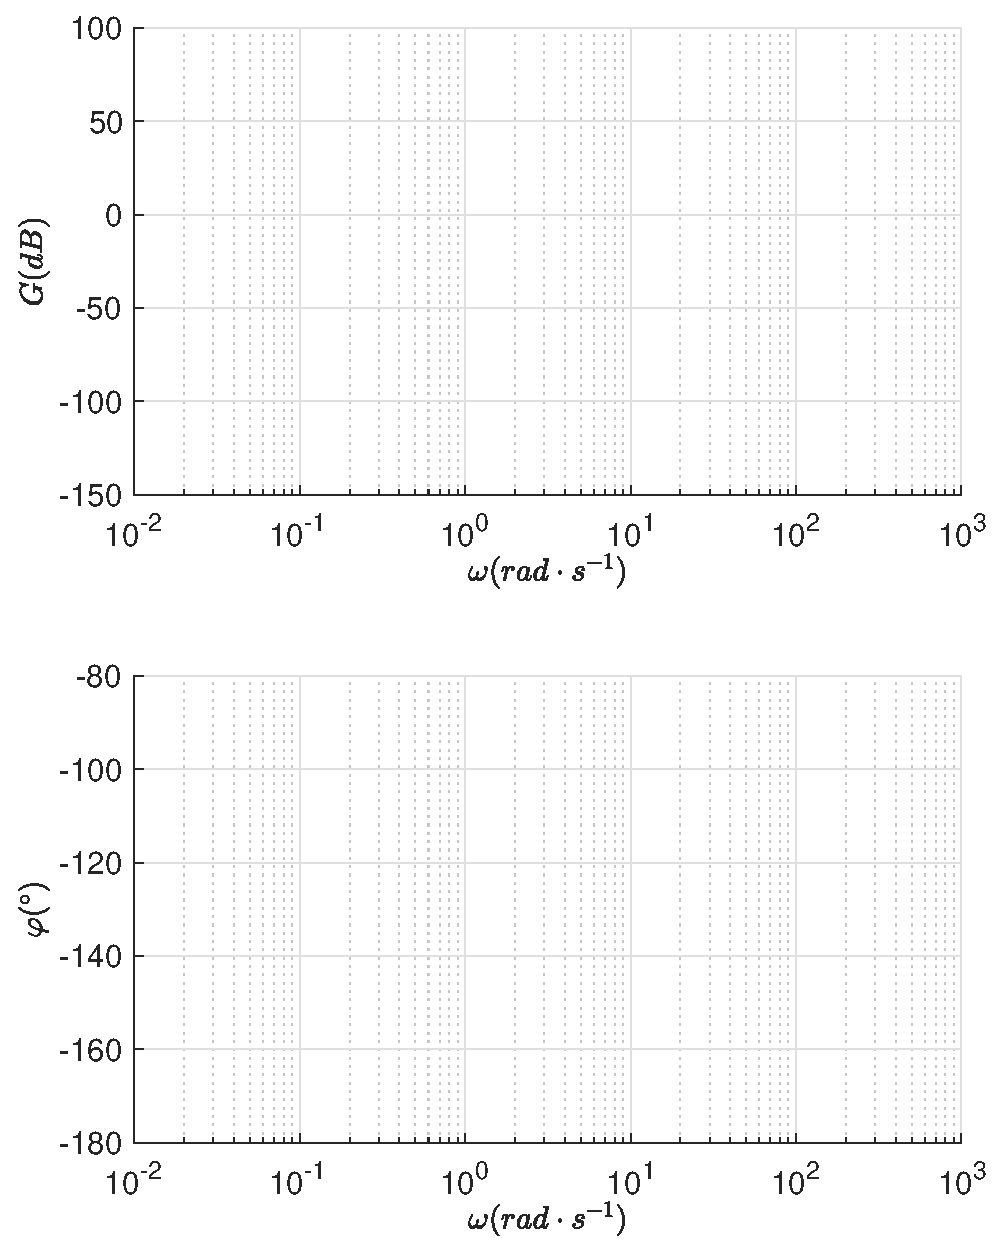
\includegraphics[width=1.0\textwidth]{images/bode_total0}
 \end{center}
 }

\else

On suppose que l'utilisateur monte l'échelle à une vitesse de $0,4 \mathrm{~m} \cdot \mathrm{s}^{-1}$ et que les barreaux de l'échelle sont distants de $40 \mathrm{~cm}$.

\fi

\question{Déterminer la valeur numérique de la fréquence de sollicitation de l'Exolift.}

\ifprof
\begin{texteCache}

 A chaque changement de barreaux par l'utilisateur, on peut supposer
  que la charge supportée par l'Exolift va augmenter puisque
  l'utilisateur va relâcher le force qu'exerce une de ses mains sur
  l'échelle.

  Pour une vitesse moyenne de \(0,4\ m.s^{- 1}\), les barreaux étant
  espacés de \(0,4\ m\), il y aura un changement de barreau toute les
  \(\frac{0.4}{0,4} = 1s\), soit une fréquence de 1 Hz.

 
 \vspace{1.5cm}

\end{texteCache}
\else


\fi

\question{Quel sera le comportement de l'Exolift soumis à cette sollicitation? Conclure sur le respect de l'exigence 1.3.2.}

\ifprof
\begin{texteCache}

 A une pulsation de \(\omega=2\pi\cdot f\approx 6,3\ \text{rad.}s^{- 1}\) (1Hz), aucune résonance
  n'est observée, ce qui valide l'exigence 1.3.2.

 
 \vspace{1.5cm}

\end{texteCache}
\else


\fi

%
%\section{Partie IV - Assurer la sécurité du technicien}
%Objectif : déterminer les contraintes liées au montage de la sangle (exigence 1.3.3).
%
%Une fois l'opération de pesée réalisée et l'action de montée/descente enclenchée par le technicien, l'Exolift va fournir la puissance nécessaire pour supporter une partie de la charge. Le moteur électrique transmet sa puissance mécanique de rotation à un galet par le biais d'un réducteur/renvoi d'angle. Par l'adhérence entre le galet et la sangle installée sur l'échelle, l'ensemble \{Exolift + utilisateur\} va se translater le long de l'échelle.
%
%\section{Hypothèses et notations}
%La figure 16 présente le paramétrage de l'étude.
%
%\begin{itemize}
%  \item Les masses et inerties des galets de renvoi et de la sangle seront négligées.
%
%  \item La base d'étude $(\vec{x}, \vec{y}, \vec{z})$ est orthonormée directe.
%
%  \item L'étude se fera dans le sens de la montée à la vitesse constante $V$ (le galet motorisé tourne alors dans le sens direct) par rapport à l'échelle considérée comme référentiel galiléen.
%
%  \item Le galet, de rayon $R_{g}$, est en liaison pivot d'axe $(O, \vec{y})$ avec le corps de l'Exolift. Il est entraîné en rotation par l'ensemble moto-réducteur.
%
%  \item Le contact galet/sangle se fait avec frottement de coefficient $f$.
%
%  \item Toutes les autres liaisons sont supposées parfaites.
%
%  \item $\overrightarrow{\mathrm{d} F}=\mathrm{d} F_{n} \vec{n}+\mathrm{d} F_{t} \vec{t}$ est la force élémentaire exercée par le galet sur l'élément de sangle d'angle élémentaire $\mathrm{d} \theta$ où $\mathrm{d} F_{n}$ est la composante normale au contact et $\mathrm{d} F_{t}$ la composante tangentielle. Soit $\left\{\mathrm{d} \mathcal{T}_{g \rightarrow s}\right\}=\left\{\begin{array}{l}\overrightarrow{\mathrm{d} F} \\ \overrightarrow{0}\end{array}\right\}_{M}$ le torseur des actions mécaniques élémentaires exercées par le galet motorisé sur l'élément de sangle d'angle élémentaire $\mathrm{d} \theta$.
%
%  \item Les forces $\vec{T}$ et $\overrightarrow{T+\mathrm{d} T}$ correspondent respectivement aux actions mécaniques exercées par les brins mou et tendu de la sangle sur l'élément de sangle étudié. Ces forces sont normales aux sections droites de la sangle, paramétrées par les vecteurs unitaires $\overrightarrow{u_{1}}$ et $\overrightarrow{u_{2}}$.
%
%  \item L'angle d'enroulement total de la sangle sur le galet, noté $\alpha$, est assuré par la présence de deux galets de renvoi de centres respectifs $A$ et $B$. Ces galets de renvoi sont en liaison pivot avec le corps de l'Exolift d'axes respectifs $(A, \vec{y})$ et $(B, \vec{y})$.
%\includegraphics[width=0.9\textwidth, center]{2023_10_30_d11e80da56f59e3b3cdfg-15}
%
%\end{itemize}
%
%Figure 16 - Paramétrage local du contact galet/sangle
%
%Q31. En isolant un galet de renvoi et la partie de la sangle en contact avec lui, montrer que le galet de renvoi ne modifie pas la valeur de la tension dans la sangle.
%
%Q32. Montrer que le moment élémentaire des actions mécaniques du galet motorisé sur la sangle au point $O$ s'écrit $\overrightarrow{\mathrm{d}} \overrightarrow{\mathcal{M}_{O}}=R_{g} \mathrm{~d} F_{t} \vec{y}$.
%
%Pour la Q33, on considère que la portion de sangle en contact avec le galet est indéformable. On note $\omega_{s}$ et $\omega_{g}$ les vitesses de rotation respectives de la portion de sangle et du galet par rapport à l'Exolift autour de l'axe $(O, \vec{y})$.
%
%La suite de l'étude se fait à la limite d'adhérence entre la sangle et le galet.
%
%Q33. Déterminer la vitesse de glissement au point $M$ de la sangle par rapport au galet motorisé, notée $\vec{V}_{M, s / g}$, en fonction de $\omega_{s}$ et de $\omega_{g}$. Justifier alors le sens de l'effort tangentiel $\mathrm{d} F_{t}$.
%
%Q34. D'après la loi de Coulomb et dans les hypothèses d'étude, donner la relation entre $\mathrm{d} F_{n}$ et $\mathrm{d} F_{t}$.
%
%Q35. En précisant le principe ou théorème appliqué sur l'élément de sangle, déterminer les relations qui relient les différents efforts aux paramètres du problème et en déduire l'expression des deux composantes élémentaires $\mathrm{d} F_{n}$ et $\mathrm{d} F_{t}$.
%
%Q36. Montrer qu'une linéarisation (développement limité) à l'ordre 1 permet d'obtenir le système linéaire suivant :
%
%$$
%\left\{\begin{array}{l}
%\mathrm{d} F_{n}=T \mathrm{~d} \theta \\
%\mathrm{d} F_{t}=-\mathrm{d} T
%\end{array}\right.
%$$
%
%Q37. En utilisant la relation obtenue à la Q34, déterminer l'expression de $T(\theta)$, tension dans la sangle à l'angle d'enroulement $\theta$, en fonction du poids $P_{\text {tot }}$ de l'ensemble à soulever appliqué à la sangle tel que $T\left(\theta=\theta_{\text {min }}\right)=P_{\text {tot }}$.
%
%Q38. En déduire l'expression littérale du couple transmissible $C_{t}$ par adhérence du galet sur la sangle à la limite de l'adhérence en fonction de $R_{g}, P_{t o t}, f$ et de $\alpha$.
%
%Les courbes de la figure 17 présentent les évolutions de la tension dans le brin mou de la sangle à la limite de l'adhérence pour différents efforts dans le brin tendu en fonction de l'angle d'enroulement total $\alpha$. L'angle d'enroulement adopté par le constructeur est de $232^{\circ}$.
%\includegraphics[width=0.9\textwidth, center]{2023_10_30_d11e80da56f59e3b3cdfg-16}
%
%Figure 17 - Évolution de la tension du brin mou dans la sangle en fonction de l'angle d'enroulement de la sangle sur le galet pour différents efforts dans le brin tendu
%
%Q39. À partir de la figure 17, justifier l'utilisation d'un contre-poids à fixer sur l'extrémité basse du brin mou de la sangle.
%
%L'ensemble contre-poids est composé d'une portion de sangle, de longueur de $2 \mathrm{~m}$ et de masse linéïque de $0,07 \mathrm{~kg} \cdot \mathrm{m}^{-1}$, et d'une masse de $4 \mathrm{~kg}$ suspendue à cette portion de sangle.
%
%Q40. Déterminer l'effort dans le brin mou de la sangle.
%
%Q41. En déduire l'angle d'enroulement nécessaire au respect de l'exigence 1.3.3 sachant que l'Exolift a une masse de $12 \mathrm{~kg}$. Valider alors le choix de l'angle d'enroulement du constructeur.
%
%Q42. Le constructeur a choisi d'utiliser un réducteur irréversible. Justifier ce choix vis-à-vis de la sécurité de l'utilisateur.
%
%\section{FIN}
%\begin{center}
%\includegraphics[width=0.9\textwidth]{images/2023_10_30_d11e80da56f59e3b3cdfg-17(1)}
%\end{center}
%
%\section{DOCUMENT RÉPONSE}
%Ce Document Réponse doit être rendu dans son intégralité avec la copie.
%
%DR1 - Chaîne structurelle de l'Exolift
%
%Q1
%
%\begin{center}
%\includegraphics[width=0.9\textwidth]{images/2023_10_30_d11e80da56f59e3b3cdfg-17}
%\end{center}
%
%Exolift en mouvement
%
%\section{DR2 - Opération de pesée}
%Q5 Pour remplir les couleurs des leds allumées, noircir les leds allumées en vert, faire une croix sur celles allumées en rouge et ne pas modifier les leds éteintes. L'exemple ci-contre représente le cas où la led 1 est allumée en vert, la led 3 est allumée en rouge et les autres leds sont éteintes.
%
%\begin{center}
%\includegraphics[width=0.9\textwidth]{images/2023_10_30_d11e80da56f59e3b3cdfg-18}
%\end{center}
%
%\begin{center}
%\begin{tabular}{|c|c|c|c|c|c|}
%\hline
%instants & $t=0 \mathrm{~s}$ & $t=1 \mathrm{~s}$ & $t=2 \mathrm{~s}$ & $t=3 \mathrm{~s}$ & $t=4 \mathrm{~s}$ \\
%\hline
%leds &  &  &  &  &  \\
%\hline
%Pmes & 0 & 0 &  &  &  \\
%\hline
%défaut & 0 & 0 &  &  &  \\
%\hline
%instants & $t=5 \mathrm{~s}$ & $t=6 \mathrm{~s}$ & $t=7 \mathrm{~s}$ & $t=8 \mathrm{~s}$ & $t=9 \mathrm{~s}$ \\
%\hline
%\multicolumn{6}{|l|}{leds} \\
%\hline
%\multicolumn{6}{|l|}{Pmes} \\
%\hline
%\multicolumn{6}{|l|}{défaut} \\
%\hline
%instants & $t=10 \mathrm{~s}$ & $t=11 \mathrm{~s}$ & $t=12 \mathrm{~s}$ & $t=13 \mathrm{~s}$ & $t=14 \mathrm{~s}$ \\
%\hline
%\multicolumn{6}{|l|}{leds} \\
%\hline
%\multicolumn{6}{|l|}{Pmes} \\
%\hline
%défaut &  &  &  &  &  \\
%\hline
%\end{tabular}
%\end{center}
%
%DR3 - Filtrage par moyenne glissante
%
%Q11
%
%\begin{center}
%\begin{tabular}{cccccc}
%\hline
%$i$ & 0 & 1 & 2 & 3 & 4 \\
%\hline
%$u_{i}$ & -2 & 0 & -1 & 2,5 & 3 \\
%\hline
%$u_{i}^{f}$ &  &  &  &  &  \\
%\hline
%\end{tabular}
%\end{center}
%
%DR4 - Schéma-blocs associé au modèle de comportement de l'Exolift
%
%Q22
%
%\begin{center}
%\includegraphics[width=0.9\textwidth]{images/2023_10_30_d11e80da56f59e3b3cdfg-19}
%\end{center}
%
%DR5 - Diagrammes de Bode associés au comportement de l'Exolift
%
%Q28
%\includegraphics[width=0.9\textwidth, center]{2023_10_30_d11e80da56f59e3b3cdfg-19(1)}
%

\FloatBarrier

\ifprof

\else
\subsection{D6 - Diagramme d'exigences extrait du cahier des charges de l'Exolift}

\begin{figure}[!htb]
\begin{center}
\includegraphics[width=0.9\textwidth]{images/2023_10_30_d11e80da56f59e3b3cdfg-20}
\caption{Diagramme d'exigences extrait du cahier des charges de l'Exolift \label{DR6}}
\end{center}
\end{figure}

\fi

